\documentclass{article}
\usepackage[a4paper, total={15cm, 24cm}]{geometry}
\usepackage[utf8]{inputenc}
\usepackage{listings}
\usepackage{color}
\usepackage{rotating}
\usepackage{setspace}

\usepackage{graphicx}
\usepackage{subfig}

\definecolor{codecolour}{rgb}{0.1,0.1,0.1}
\definecolor{commentcolour}{rgb}{0.5,0.5,0.5}
\definecolor{codegray}{rgb}{0.5,0.5,0.5}
\definecolor{codepurple}{rgb}{0.58,0,0.82}
\definecolor{backcolour}{rgb}{1,1,1}

\lstset{
    backgroundcolor=\color{backcolour},
    commentstyle=\color{commentcolour}\textit,
    keywordstyle=\color{magenta},
    numberstyle=\tiny\color{codegray},
    stringstyle=\color{codepurple},
    basicstyle=\small\color{codecolour},
    tabsize=2,
    numbers=left,
    stepnumber=1,
}

\graphicspath{ {plot/} }
\begin{document}
\thispagestyle{plain}
\topskip0pt
\vspace*{\fill}
\begin{center}

    \begin{Huge}
    \textbf{Sorch}
    \end{Huge}
    \vspace{1cm}

    Un algoritmo di ricerca che riduce il disordine del campione.
    \vspace{1cm}

    Progetto finale per il corso di Algoritmi e Strutture di Dati.
    \vspace{1cm}

    \begin{Large}
    \textbf{Giles Sebastian}
    \end{Large}
    \vspace{1cm}

    Matricola: 1071522
    \vspace{0.4cm}

    E-mail: s1071522@studenti.univpm.it
    \vspace{0.4cm}

    Maggio 2017

\end{center}
\vspace*{\fill}

\newpage
\setstretch{1.16}
\section{L'idea}

    \textit{Ordinare un vettore per poi sfruttare la ricerca dicotomica,
    oppure usare una semplice ricerca lineare?}

    La scelta dipende dalla dimensione della popolazione e dal numero
    di ricerche che si prevede di fare.
    L'algoritmo “sorch” (\textit{sort-search}) fornisce un buon compromesso tra
    il pesante costo iniziale per l'ordinamento e la lentezza di una ricerca
    lineare.

    L'idea di fondo è quella di ottenere una progressiva riduzione dei tempi
    di ricerca all'aumentare del numero di ricerche effettuate, contribuendo
    ognuna di esse a dare uno pseudo ordinamento al vettore.

\section{L'algoritmo}

    La prima ricerca è necessariamente di impronta lineare essendo il vettore
    disordinato.
    La ricerca lineare classica compie $n$ confronti solo nel caso
    peggiore, questo algoritmo invece impone di percorrere l'intero vettore in
    modo da partizionarlo (come per il primo passo di quicksort).

    Compiere simultaneamente ricerca e partizionamento in un unico ciclo
    permette di sfruttare i confronti con il pivot per ridurre (in media
    dimezzare) il numero di confronti di uguaglianza richiesti per la ricerca.

    Alla fine della prima ricerca il vettore sarà partizionato rispetto ad un
    pivot.

    Alla chiamata successiva, l'azione di ricerca e partizionamento viene
    ripetuta sul sottoinsieme opportunamente a sinistra o destra del pivot in
    base al confronto dell'elemento cercato con il pivot stesso. Il risultato
    del partizionamento è un secondo pivot che divide ulteriormente il vettore.

    Questa procedura si presta alla \textbf{ricorsione}.

    È necessario un meccanismo che tenga traccia dei partizionamenti svolti, al
    fine di trarne vantaggio nella fase di \textit{divide} delle ricerche
    successive, basata sul confronto dell'elemento cercato con i pivot. La
    struttura di dati più naturale per questo scopo è un albero binario di
    ricerca.

    La radice di questo albero (\textit{albero degli indici}) deve essere
    inizializzata con il \textbf{puntatore al primo elemento} del vettore da
    “indicizzare” e la sua \textbf{lunghezza}, il puntatore al pivot viene
    inizializzato a NULL, per indicare che la partizione non è ancora stata
    fatta.

    Il \textit{caso base}, e quindi la chiusura della ricorsione, può avere 3
    casi:
    \begin{enumerate}
    \item Se il puntatore al pivot è NULL \textbf{avviene un partizionamento con
      simultanea ricerca.} Alla fine di ogni partizionamento la posizione del
      pivot viene memorizzata sul nodo e vengono aggiunte due foglie, figlie di
      questo nodo, rispettivamente per le partizioni sinistra e destra.

      Ogni foglia appena creata viene inizializzata nello stesso modo della
      radice dell'albero, considerando il puntatore al primo elemento della
      corrispondente partizione e la sua lunghezza.

      Se nel blocco appena partizionato non ci fossero elementi minori (risp.
      maggiori) del pivot, durante la creazione della foglia sinistra (risp.
      destra) viene riconosciuta la lunghezza 0 della partizione e viene
      assegnato un puntatore NULL. Questo avviene in particolare quando tutti
      gli elementi adiacenti nel vettore sono diventati dei pivot e cioè il
      vettore è completamente indicizzato (e ordinato) su un intervallo.

      Se l'elemento cercato fosse stato trovato ne viene ritornato il puntatore,
      altrimenti NULL.

    \item \textbf{Viene ritornato immediatamente NULL.} Se l'albero è NULL
      quanto avviene nel caso 1 garantisce che il vettore sia completamente
      ordinato in un intorno del punto in cui ci si aspetta di trovarlo, ma
      l'elemento non c'è.

    \item \textbf{Viene ritornato immediatamente il puntatore al pivot} qualora
      questo coincida con l'elemento cercato.
    \end{enumerate}

\section{Alcune misurazioni}
    I grafici in appendice sono stati disegnati usando Matlab. I dati sono stati
    ottenuti con un programma in C che ha eseguito ricerche ripetute con i tre
    algoritmi su diversi campioni casuali misurandone il tempo impiegato.

    In ordinata compare il tempo accumulato per compiere il numero di ricerche
    in ascissa. Per il metodo dicotomico questo include il tempo richiesto per
    l'ordinamento iniziale.

    Tutte le curve sono state ottenute facendo la media dei risultati per 10
    popolazioni diverse, ognuna costitutita dai primi $n$ numeri naturali,
    ogni volta disordinati casualmente.

    Le query di ricerca sono generate casualmente in maniera uniforme.

    In azzurro, arancione e giallo si hanno rispettivamente le curve per ricerca
    lineare, ricerca dicotomica e sorch.

    \begin{itemize}
      \item \textbf{Figura 1} $n = 10^5$, $10^2$ query prese uniformemente su
        tutto il campione.

        È visibile la superiorità della ricerca lineare per le prime ricerche.

      \item \textbf{Figura 2} $n = 10^5$, $10^4$ query prese uniformemente su
        tutto il campione.

        È visibile il vantaggio a lungo termine ottenuto dall'ordinamento.

      \item \textbf{Figura 3} $n = 10^5$, $10^2$ query prese uniformemente
        sull'intervallo $[4.5*10^4, 5.5*10^4]$

        L'algoritmo sorch è molto performante quando le query sono vicine tra
        loro rispetto alla dimensione del campione, questo è dovuto ad una fitta
        indicizzazione sull'intervallo interessato.

      \item \textbf{Figura 4} $n = 10^3$, $10^2$ query prese uniformemente su
        tutto il campione.

        Quando il campione è ristretto l'ordinamento costa poco e viene ripagato
        subito. L'algoritmo sorch rimane indietro a causa dell'overhead per la
        gestione dell'albero degli indici.

    \end{itemize}
\setstretch{1}
\section{Codice C}
\lstinputlisting[language=C, lastline=24]{indexer.h}
\pagebreak
\lstinputlisting[language=C, firstnumber=26,firstline=26]{indexer.h}

\newpage
\captionsetup[subfigure]{labelformat=empty}
\begin{sidewaysfigure}
  \centering
  \subfloat[Figura 1]{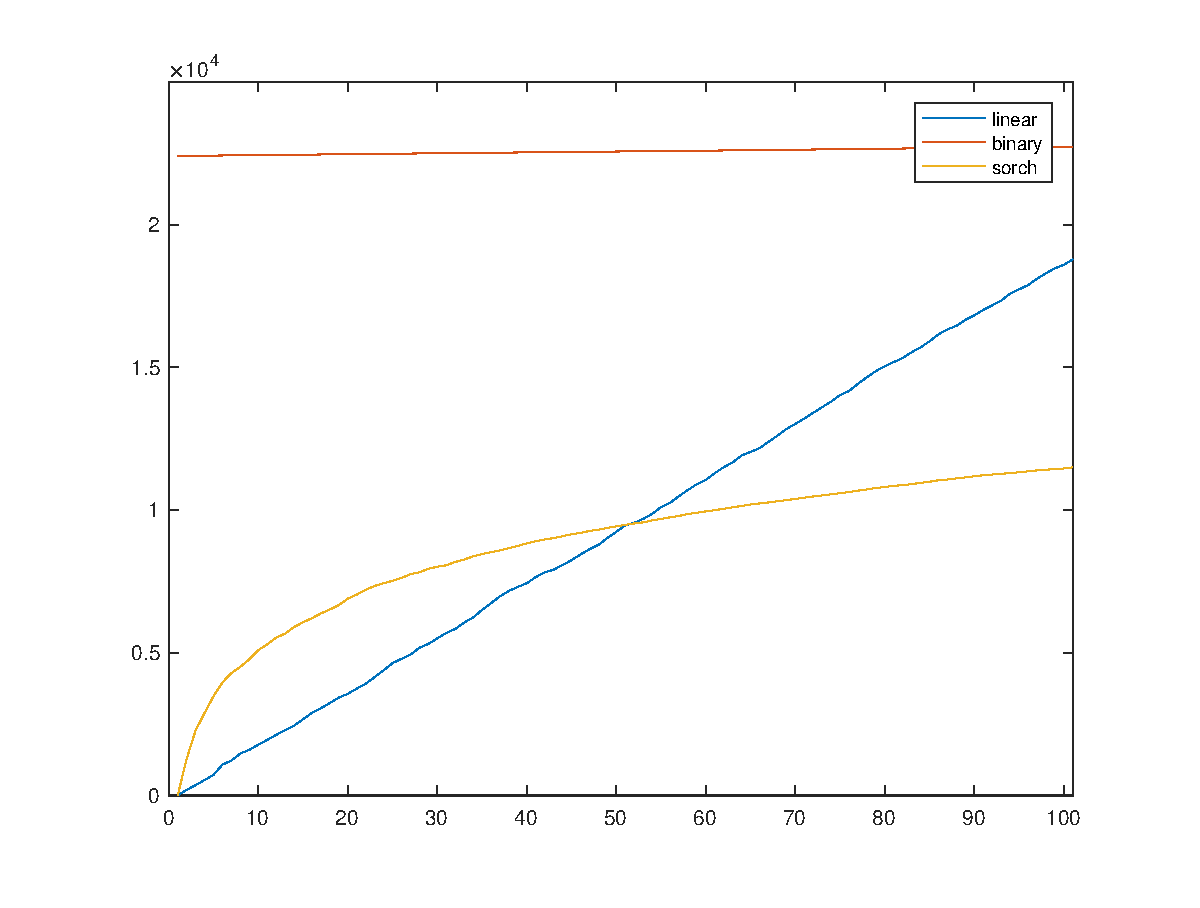
\includegraphics[width=0.45\textheight]{standard.eps}}
  \subfloat[Figura 2]{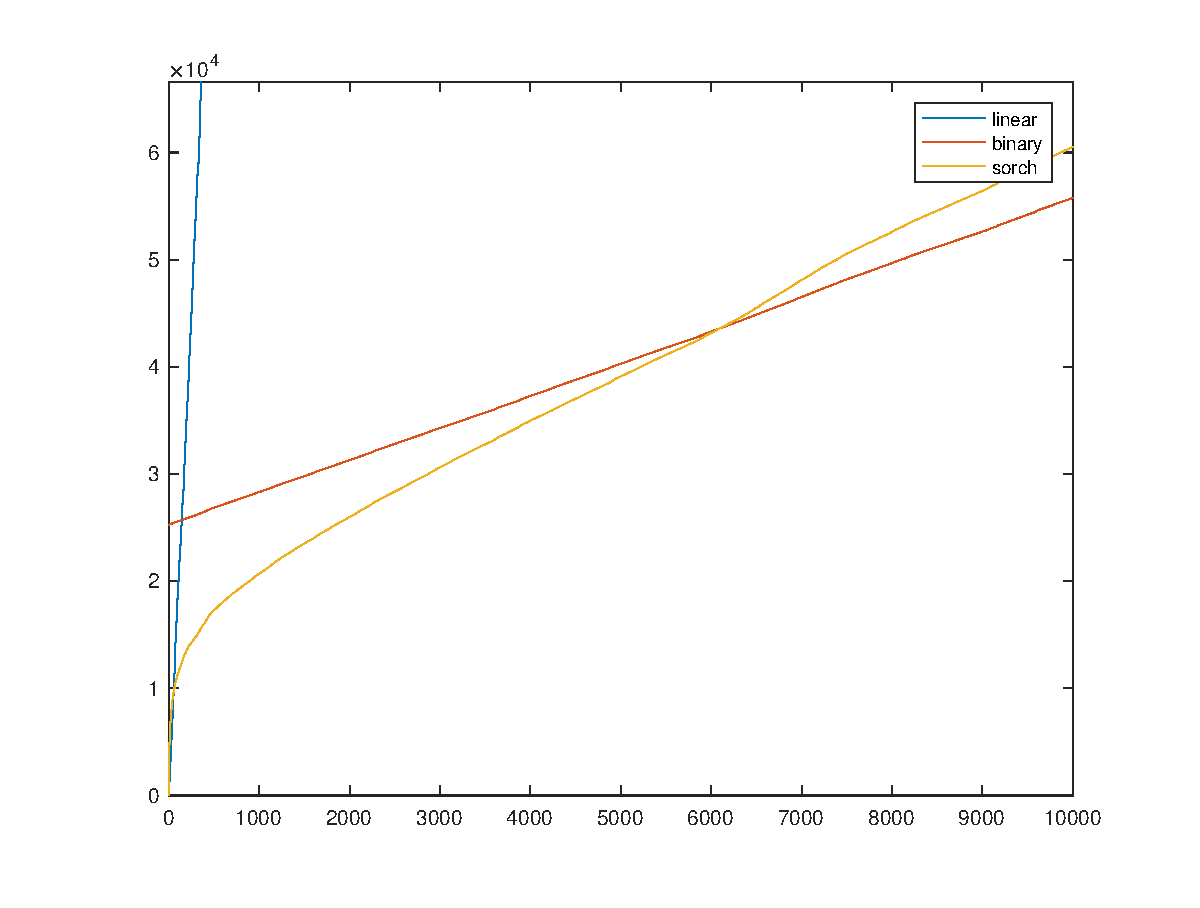
\includegraphics[width=0.45\textheight]{manysearches.eps}}

  \subfloat[Figura 3]{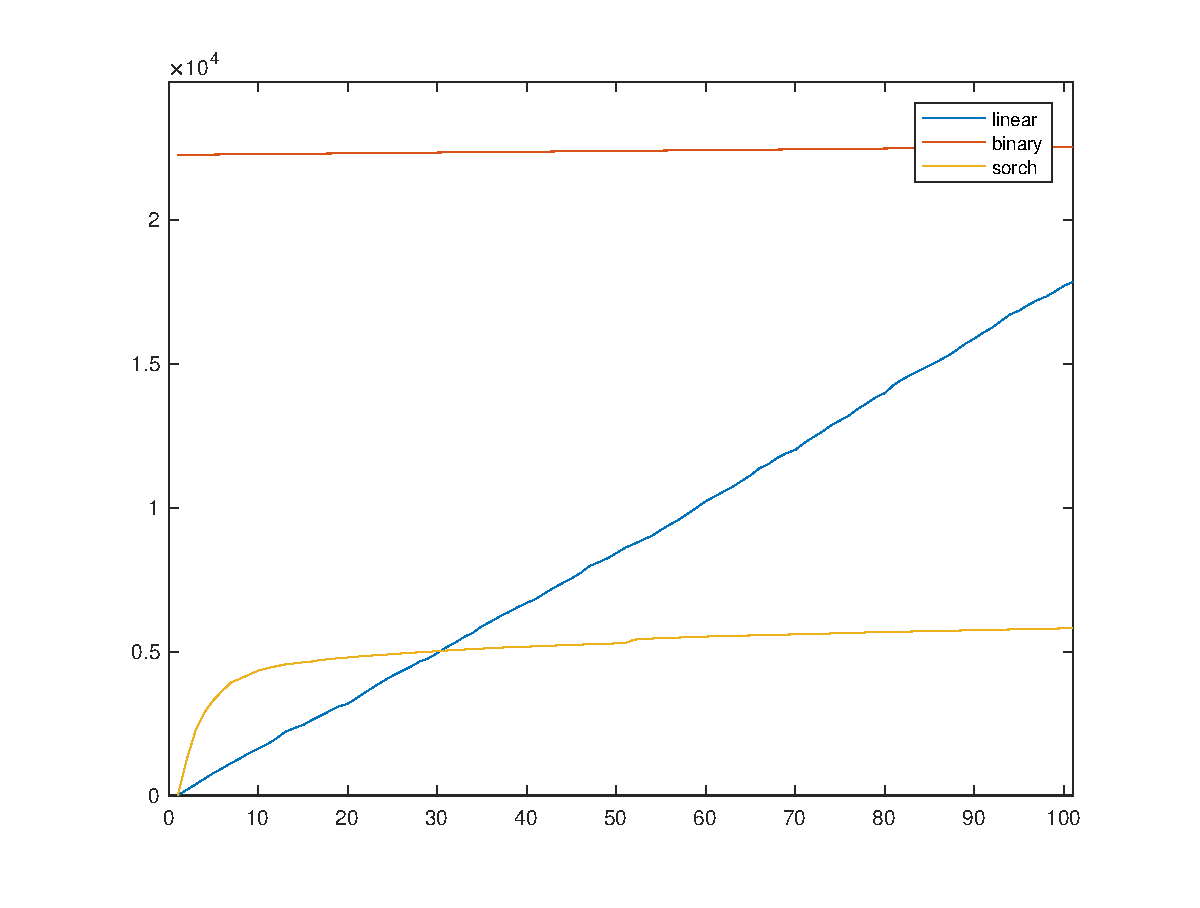
\includegraphics[width=0.45\textheight]{restrictedsearches.eps}}
  \subfloat[Figura 4]{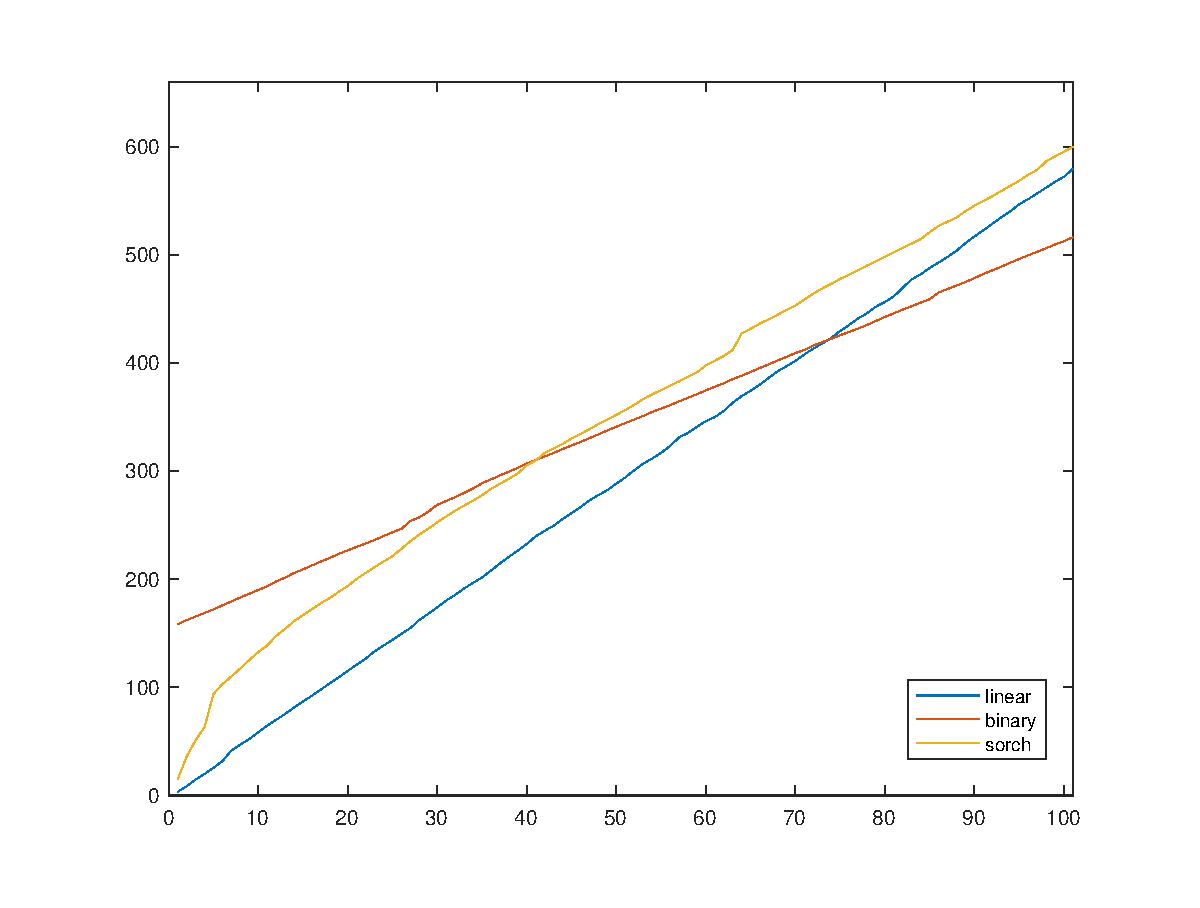
\includegraphics[width=0.45\textheight]{fewdata.eps}}
\end{sidewaysfigure}
\end{document}
